\section{ОБЗОР ЛИТЕРАТУРЫ}\label{sec:overview}
\subsection{Обзор аналогов}\label{subsec:overview:overview_analogue}
Крупнейшими продуктами на рынке анализа тональности текста для множества естественных языков являются: Natural Language API, поставляемый на Google Cloud Platform; Text Analysis API, поставляемый на платформе Microsoft Azure; IBM Watson; WIT.AI принадлежащий Facebook. Данные решения представляют собой облачные сервисы, предоставляющие API пользователям, которое позволяет загружать тексты на естественных языках и возвращает их анализ. Кроме анализа тональности эти сервисы предоставляют и другие возможности, как определение частей речи (Part of Speech Tagging, PoS Tagging), морфологический разбор слов и синтаксический разбор предложений. Такие системы носят название NLP-конвейера (Natural Language Processing). К сожалению исходные коды этих систем закрыты, а применяемые в них принципы если и распространяются, то описаны в платных научных изданиях. Однако можно уверенно предположить, что Google применяет Globally Normalized Transition-Based Neural Networks\cite{google_gntb}. Так как реализацию  данного подхода Google анонсировал в виде мощного и высокопроизводительного NLP инструмента SyntaxNet.

Так же стоит обратить внимание на крупный академический проект от Стенфодрского университета --- CoreNLP\@. CoreNLP --- это открытый NLP конвейер, демонстрирующий практические возможности методов, изобретенных в результате широкого ряда исследований сотрудников Стенфорда.

Итак, вне зависимости от огласки принципов работы NLP-конвейеров, все ещё можно сравнить их бизнес-логику. Сравнение возможностей описанных выше закрытых коммерческих проектов друг с другом возможно только в ходе мощного маркетингово исследования. Но если сравнить их с некоммерческим CoreNLP, то станет очевидно, что CoreNLP, являясь лишь демонстрацией, очень отстает по производительности, но предоставляет более детальную визуализацию анализа тональности. CoreNLP в результате анализа предложения выдает синтаксическое дерево, узлами которого являются слова, а ветвями --- синтаксические связи между словами. Таким образом каждое поддерево представляет собой фразу. И оценка тональности указывается для каждого узла. То есть, потенциальный пользователь может легко понять каким образом давалась оценка тональности всего предложения, глядя на оценки отдельных фраз. Коммерческие же продукты такой возможности не предоставляют, так как дают оценку всему предложению целиком в силу своей структуры. Таким образом, задача проектирования в создании модели с высокими возможностями визуализации, с использованием высокопроизводительных технологий.
\subsection{Процесс выделения особенностей}\label{subsec:overview:overview_feature_extraction}
Обычно задачи, связанные с классификацией текстов, можно разделить на три этапа: выделение особенностей, сжатие предложений и классификация. На первом этапе из текста выбирают слова для обработки и выбирают соответствующие им векторы. Затем производят сжатие набора векторов соответствующих словам в предложении в один вектор, который будет представлять все предложение. И далее полученные векторы предложений классифицируют.\cite{Goodfellow-et-al-2016}
Для классификации предложений выделение особенностей начинают со статической обработки текста, например убирают символы переноса строки, или заменяют символы, которые могут использоваться в формате представления набора данных, на аналоги или ключевые слова. Часто используется замена символов круглых скобок на сокращения ``--LRB--'' и ``--RRB--''. С этим легко справится механизм регулярных выражений. Затем необходимо разбить предложения на единицы языка, несущие независимое семантическое значение --- произвести токенизацию. Для большинства языков регулярные выражения так же справятся с задачей. Для русского языка хватит разбиения по символу пробела, в английском надо будет учитывать ещё и апострофы (``It's'' разобьется на ``It'' и ``'s''). Однако для обработки большинства восточных языков так же приходится прибегать к машинному обучению, так как синтаксическое разделение слов на письме часто отсутствует, и токенизацию можно произвести только анализируя семантическое значение предложения. Для ограничения масштаба в данной работе методы токенизации рассматриваться не будут.\cite{Goodfellow-et-al-2016}
В работе для токенизации и синтаксического разбора будут использованы средства CoreNLP встроенные в библиотеку NLTK для Python.

Итак, после токенизации предложения представляют из себя набор единиц языка в строковом формате. Но нейронные сети работают только с числами. Поэтому необходимо представить слова в векторном виде. Данный процесс называется \textit{встраивание слов}. Классический метод one-hot-encoding предлагает представлять слова в виде позиционных кодов. Для всех уникальных слов в корпусе строится словарь, где каждому слову соответствует вектор заполненный нулями и одной единицей, соответствующей позиции слова в словаре. Очевидно, это очень производительный метод встраивания слов, так как алгоритм кодирования слов в новом корпусе имеет линейную сложность. Однако прямая зависимость размера вектора от количества уникальных слов в корпусе может вызвать проблемы с хранением этих векторов. Например, корпус книг от Google содержит 1 миллион уникальных слов, и с one-hot-encoding каждое слово будет занимать 30 мегабайт памяти, если пользоваться в вычислениях хотя бы 32-битными числами. Так же семантическое значение слов в данном методе теряется --- сравнение синонимов, антонимов и никак не связанных между собой по значению слов даст один и тот же результат. Метод сжатия векторов слов в единый вектор, соответствующий предложению, заключается в простом суммировании векторов слов и носит название Мешок слов. Пример мешков слов представлен на рисунке~\ref{fig:overview:bag_of_words}\cite{Goodfellow-et-al-2016}.

\begin{figure}
\centering
  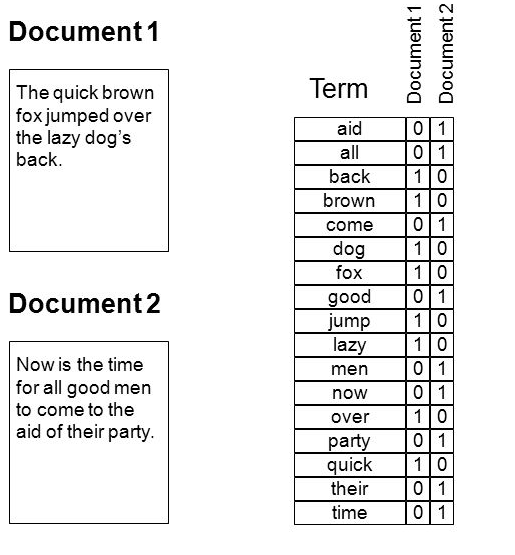
\includegraphics[height=10cm]{bag_of_words.png}
  \caption{Пример мешков для двух предложений}\label{fig:overview:bag_of_words}
\end{figure}

Скалярное произведение двух таких векторов предложений даст степень схожести этих предложений, основывающейся только на количестве одинаковых слов встречающихся в обоих предложениях. Таким образом данный метод для трех предложений ``Мальчик ударил мяч.'', ``Мальчик ударился в учебу'' и ``Дети играют в футбол'' сделает вывод о том, что схожи первые два предложения, хотя очевидно что по смыслу больше связаны первое и третье. Обучение нейронной сети на выборке из мешков слов не даст никаких результатов для задач классификации по значению не только по причине отсутствия семантики в векторных представлениях слов и фраз, но и из-за представления в виде позиционных кодов, когда большая часть вектора не несет никакой нагрузки, а содержит лишь ноли.\cite{Goodfellow-et-al-2016}
\subsection{Технология word2vec}\label{subsec:overview:overview_word2vec}
Существует ряд методов встраивания слов, в которых векторы сохраняют семантическое значение обрабатываемых слов. В основе этих методов лежит идея о том, что семантика слова заключена в контексте его применения. Самым значимым результатом исследований на почве этой идеи является технология word2vec. На сегодняшний день это самый распространенный и эффективный метод встраивания слов. Качественно обученная модель word2vec представляет собой словарь, в котором словам соответствуют так называемые плотные вектора.\cite{word2vec}

Процесс обучения модели word2vec начинается с генерации произвольных значений векторов для изучаемых слов. Каждому слову будет соответствует два плотных вектора, так как слово в процессе обучения может участвовать в роли центрального слова, и в роли слова из контекста центрального слова. На каждом шаге обучения в тексте последовательно выбирается центральное слово и его контекст --- слова которые отстоят от центрального на m слов слева и справа. Для каждого центрального слова t делается предсказание слов в контексте.\cite{word2vec} Целевой функцией оптимизации в данном случае будет

\begin{equation} \label{eq:overview:word2vec:Jprime}
  J^{\prime}(\Theta) = \prod_{t=1}^{T}\prod_{\substack{-m\leq j \geq m\\j \neq 0}}p(w_{t+j}|w_{t};\Theta),
\end{equation}
\begin{explanationx}
\item [где] $ \Theta $ --- это параметры модели, изменяемые в ходе обучения.
\end{explanationx}


Тогда отрицательная логарифмическая функция максимального правдоподобия $ J(\Theta) $ будет равна:

\begin{equation} \label{eq:overview:word2vec:J}
  J(\Theta) = -\frac{1}{T}\sum_{t=1}^{T}\sum_{\substack{-m\leq j \geq m\\j \neq 0}}\log(p(w_{t+j}|w_{t})).
\end{equation}

Для предсказания вероятности слова в контексте применяется функция softmax, описанная в общем виде в выражении

\begin{equation}
  \label{eq:overview:softmax}
  {\sigma(z)}_i = \frac{e^{z_i}}{\sum_{k=1}^{K}e^{z_k}}.
\end{equation}

Вероятность нахождения слова $o$ в контексте слова $c$ --- это softmax функция для $c$ по $o$

\begin{equation}
  \label{eq:overview:word2vec:contex_prob}
  p(o|c) = \frac{\exp({u_{o}^T}\cdot{v_{c}})}{\sum_{w=1}^{V}\exp({u_w^T}\cdot{v_{c}})}.
\end{equation}

Матрица $U$ хранит вектора в для слов из контекста, а $V$ --- для центральных слов.
Градиент для обратного прохода для~\ref{eq:overview:word2vec:J} и~\ref{eq:overview:word2vec:contex_prob} будет равен:

\begin{equation}
  \frac{\partial }{\partial v_c}\frac{\exp({u_{o}^T}\cdot{v_{c}})}{\sum_{w=1}^{V}\exp({u_w^T}\cdot{v_{c}})} = u_o - \sum_{x=1}^{V}p(x|c)\cdot{u_x}.
\end{equation}

После того, как градиент рассчитан значение градиента отнимается от всех обучаемых параметров модели, то есть от матриц $U$ и $V$.

\begin{figure}[h]
\centering
  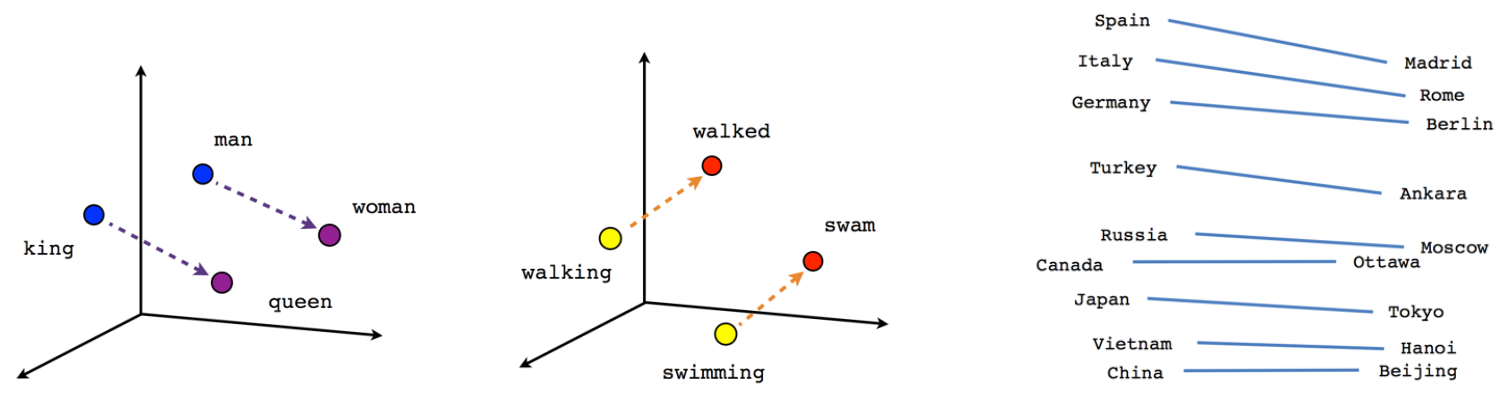
\includegraphics[height=4cm]{word2vec.png}
  \caption{Отношение между векторами в примере word2vec}\label{fig:overview:word2vec}
\end{figure}

В результате множества итераций обучения будет получена простейшая softmax модель word2vec, которая будет представлять из себя матрицу $V$. Полученные вектора хранят семантическое значение слов, таким образом близкие по смыслу слова и синонимы будут располагаться близко друг от друга. А математические операции над этими векторами будут давать интересные результаты. Например если отнять от вектора ``Король'' вектор ``Мужчина'' и добавить вектор ``Женщина'' то будет получен вектор слова ``Королева''. На рисунке~\ref{fig:overview:word2vec} видно, что вектора располагаются параллельно вдоль некоторых осей, выученных моделью, по признакам пола, части речи и географического положения. Реализовать статическую модель распознающую подобные признаки невероятно трудно.\cite{word2vec}

\subsection{Классическая рекурсивная нейронная сеть}\label{subsec:overview:rnn}
Когда каждое предложение представляет из себя набор вектор, соответствующих языковым единицам, необходимо провести сжатие --- обработать вектора слов таким образом, чтобы каждому предложению соответствовал один плотный вектор. Простейшая нейронная сеть, которая может быть применена в данной задаче --- это рекурсивная нейронная сеть (RNN). Данная сеть имеет два входа: $x_{t}$ --- входной вектор, $s_{t-1}$ --- вектор состояния с прошлой итерации. Сеть последовательно применяется к векторам в предложении слева направо, и выдает на каждой итерации выходной вектор $o_{t}$ и вектор состояния $s_t$.

\begin{figure}[h]
\centering
  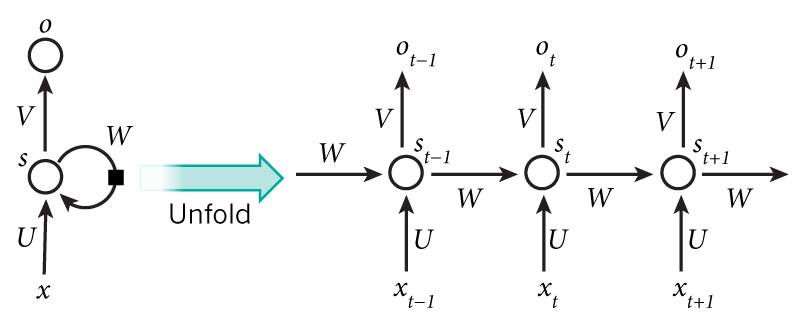
\includegraphics[height=4cm]{rnn.png}
  \caption{Рекурсивная нейронная сеть в развертке во времени}\label{fig:overview:rnn}
\end{figure}
Состоит сеть из трех матриц весов: входная матрица $U$, матрица состояний $W$, матрица выходов $V$. B описывается двумя функциями~\ref{eq:overview:rnn:state} и~\ref{eq:overview:rnn:output}. Softmax функция описана в~\ref{eq:overview:softmax}. Пример рекурсивной нейронной сети и её развертки во времени представлен на рисунке~\ref{fig:overview:rnn}.

\begin{equation}
  \label{eq:overview:rnn:state}
  s_t = f(U\cdot{x_t} + W\cdot{s_{t-1}}),
\end{equation}

\begin{equation}
  \label{eq:overview:rnn:output}
  o_t = softmax(Vs_t),
\end{equation}
\begin{explanationx}
\item [где] $f$ --- это функция активации, обычно выбирают тангенс.
\end{explanationx}

После обхода всего предложения, получается выходной вектор, и появляется возможность посчитать функцию потерь, и вычислить значение градиента. На рисунке~{fig:overview:rnn} показана развертка во рекурсивной сети во времени. Таким образом модель можно представить в виде многослойной сети. А значит модель страдает от проблемы затухающего градиента, когда градиентный спуск необходимо произвести на множество слоев вниз, и значение функции ошибки может очень сильно отличаться от реального её значения. Но так как применяется одна и та же сеть на каждом слое, то проблема затухающего градиента для рекурсивной сети усиливается. Поэтому с помощью RNN не было получено высоких результатов в классификации предложений. Так же рекурсивная сеть сталкивается с проблемой отдаленных зависимостей. Суть проблемы в том, что семантически связанные слова, которые имеют главную роль в понимании предложения, могут находиться удаленно друг от друга в предложении. И так как RNN обходит предложение слева на право, то информация о том, что первое слово встречалось в предложении может уже быть потеряно к тому моменту, как на вход придет второе, и модель сделает неверный вывод.

\subsection{Long Short Term Memory}\label{fig:overview:lstm}
Проблему отдаленных зависимостей решает нейронная сеть под названием Long Short Term Memory (LSTM). Это особый вид рекурсивной нейронной сети, способная выучить удаленные зависимости. Данное свойство было получено за счет усложнения структуры сети. Принцип применения и обучения остался таким же: предложение обходится слева направо последовательно подавая на вход сети плотные вектора соответствующие словам. Схема сети представлена на рисунке~\ref{fig:overview:lstm}.\cite{LSTM}

\begin{figure}[h]
\centering
  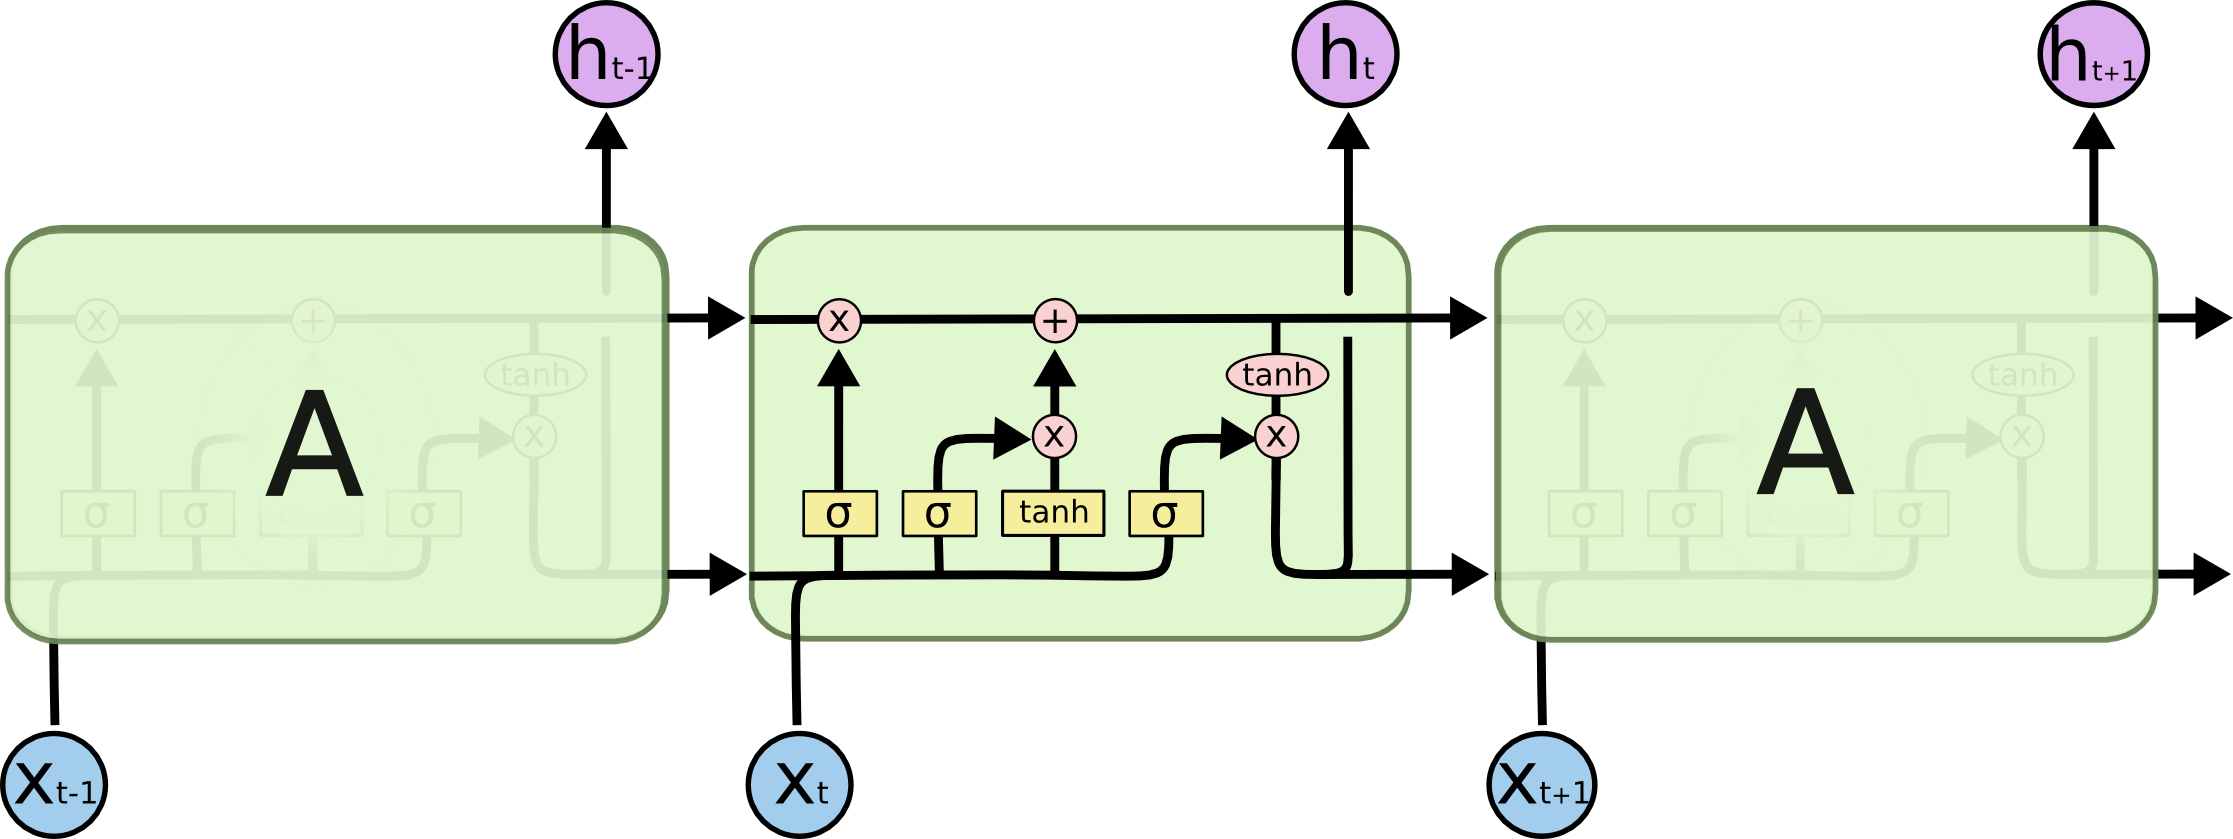
\includegraphics[height=4cm]{lstm.png}
  \caption{Схематическое изображение LSTM-сети}\label{fig:overview:lstm}
\end{figure}

Внутреннее состояние сети описывается вектором состояния ячейки $C_t$ и вектором скрытого слоя $h_t$. На вход принимает входной вектор $x_t$ и состояние с прошлой итерации: $C_{t-1}$ и $h_{t-1}$. Выходной вектор $o_t$ равен вектору скрытого слоя $h_t$. Введена система врат. Врата блокируют или пропускают векторы между различными состояниями нейронной сети. $f_{t}$ --- сигнал забывания, сбрасывает состояния ячейки. $i_{t}$ --- входные врата, блокируют или пропускают входной вектор. И $o_t$ --- выходные врата, блокируют или пропускают выходной вектор. Состояния врат описаны выражениями~\ref{eq:overview:lstm:input_gate},~\ref{eq:overview:lstm:output_gate} и~\ref{eq:overview:lstm:forget_signal}.\cite{LSTM}

\begin{equation}
  \label{eq:overview:sigmoid}
  \sigma(x) = \frac{1}{1 + e^{-x}},
\end{equation}
\begin{equation}
  \label{eq:overview:lstm:input_gate}
  i_t = \sigma(W_{i}\cdot{x_t} + U_{i}\cdot{h_{t-1}} + b_i),
\end{equation}
\begin{equation}
  \label{eq:overview:lstm:forget_signal}
  f_t = \sigma(W_{f}\cdot{x_t} + U_{f}\cdot{h_{t-1}} + b_f),
\end{equation}
\begin{equation}
  \label{eq:overview:lstm:output_gate}
  o_t = \sigma(W_{o}\cdot{x_t} + U_{o}\cdot{h_{t-1}} + b_o),
\end{equation}
\begin{explanationx}
\item [где] $\sigma$ это функция сигмоида описанная~\ref{eq:overview:sigmoid};
\item $W$ и $U$ --- это тензоры весов LSTM\@.
\end{explanationx}

Состояния ячейки вычисляются согласно выражениям~\ref{eq:overview:lstm:cell_candidate},~\ref{eq:overview:lstm:new_cell} и~\ref{eq:overview:lstm:new_hidden}.FREE FLOW FLAVA

\begin{equation}
  \label{eq:overview:hadamar}
  {(A\odot{B})}_{i,j} = {(A)}_{i,j}\cdot{{(B)}_{i,j}},
\end{equation}

\begin{equation}
  \label{eq:overview:lstm:cell_candidate}
  \tilde{C}_t = \tan(W_{C}\cdot{x_{t}} + U_{c}\cdot{h_{t-1}} + b_c),
\end{equation}

\begin{equation}
  \label{eq:overview:lstm:new_cell}
  C_t = f_t\odot{c_{t-1}} + i_t\odot{\tilde{C}_t},
\end{equation}

\begin{equation}
  \label{eq:overview:lstm:new_hidden}
  h_t = o_t\odot{\tan(c_t)},
\end{equation}
\begin{explanationx}
\item [где] $\tilde{C}_t$ носит название кандидата в состояние ячейки;
\item ${\odot}$ --- это операция произведения Адамара, описанная в~\ref{eq:overview:hadamar} для двух матриц $A$ и $B$.
\end{explanationx}

LSTM на сегодняшний день лежит в основе самой эффективной модели анализа тональности предложений Sentiment Neuron от сообщества OpenAi. Помимо лидерства на текущий момент, Sentiment Neuron обучается без учителя --- это единственная успешная модель способная сжимать вектора слов в плотный вектор предложения и обучающая без учителя. Однако обучение этой модели крайне дорого. OpenAi обучали её на четырех Nvidia Pascal Titan X и обучение заняло приблизительно один месяц.\cite{openai}

\subsection{Рекурсивная тензорная нейронная сеть}
Проблема отложенных связей может решаться иначе. Очевидно, что порядок слов в предложении редко совпадает с нитью размышлений автора. Обход предложения слева направо не может запомнить все семантически значимые последовательности, особенно в языках со специфической грамматикой. Поэтому исследователи решили изменить порядок обхода предложений. Один из итогов исследований --- это модель рекурсивной нейронной тензорной сети (RNTN), которая легла в основу CoreNLP\@. Обход предложения производится по синтаксическому дереву, построенному согласно генеративной грамматике Хомского.\cite{Chomsky}
Итак, в процесс выделения особенностей добавляется ещё один шаг --- синтаксический анализ предложения. Для RNTN необходимо на входе иметь синтаксическое дерево составляющих --- один из видов синтаксических деревьев. Это дерево удобно тем, что его можно нормализовать, то есть привести к виду бинарного дерева. На рисунке~\ref{fig:overview:constituency_tree} показан пример синтаксического дерева составляющих.\cite{Chomsky}

\begin{figure}[h]
\centering
  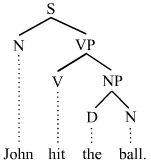
\includegraphics[height=4cm]{constituency_tree.png}
  \caption{Пример синтаксического дерева составляющих}\label{fig:overview:constituency_tree}
\end{figure}

Как видно из рисунка~\ref{fig:overview:constituency_tree}, слова представлены листьями дерева, а его узлы --- это различные виды составляющий в предложении. Типы связей не нужны в модели RNTN, интересен только сам факт их наличия и какие слова и фразы они объединяют. Для того, чтобы эффективно обрабатывать дерево составляющих, RNTN модифицирована и имеет два входа, и один выход. То есть она принимает два вектора с нижних узлов и передает верхнему, и т.д., пока в результате обработки всего дерева не будет получен один вектор, соответствующий всему предложению. Так же модель выдает вектор для каждого узла в дереве, что соответствует фразам в предложении. Это свойство эффективно применяется при обучении. Специально для обучения RNTN был создан Stanford Sentiment Treebank (SST) --- Стенфордский набор деревьев тональности. Это набор более чем из десяти тысяч синтаксических деревьев, все узлы которых оценены по тональности носителями языка. SST стал очень популярен и вне исследований RNTN и является классическим набором для измерения эффективности метода оценки тональности.\cite{RNTN}

Пусть $\begin{bmatrix}a\\b\end{bmatrix}$ --- два вектора размерности $d$ объединенные в один размерностью $2d$. Тогда значение вектора результата $p$ для входных векторов $a$ и $b$ высчитывается по формуле~\ref{eq:overview:rntn:p}.\cite{RNTN}

\begin{equation}
  \label{eq:overview:rntn:p}
  p = f(
  \begin{bmatrix}
    a\\
    b
  \end{bmatrix}^{T}\cdot{V}\cdot{
  \begin{bmatrix}
    a\\
    b
  \end{bmatrix}} + W\cdot{
  \begin{bmatrix}
    a\\
    b
  \end{bmatrix}}),
\end{equation}

\begin{explanationx}
\item [где $f$] --- функция активации;
\item $V$, $W$ --- матрицы весов модели.
\end{explanationx}

\subsection{Tree LSTM}
На следующий год после релиза RNTN, изменяется подход в синтаксическом разборе предложений, так как выходит работа с описанием алгоритма синтаксического разбора с линейной сложностью. Однако этот алгоритм возвращает дерево зависимостей, а RNTN работает с деревом составляющих. Пример дерева зависимостей представлен на рисунке~\ref{fig:overview:dependency_tree}. Дерево зависимостей несет в себе меньше информации, чем дерево составляющих, так как дерево составляющих можно сконвертировать в зависимости без потерь, а обратный процесс без потерь невозможен.\cite{Chomsky}

\begin{figure}[h]
\centering
  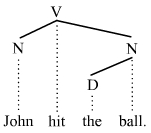
\includegraphics[height=4cm]{dependency_tree.png}
  \caption{Пример синтаксического дерева зависимостей}\label{fig:overview:dependency_tree}
\end{figure}

\begin{figure}[h]
\centering
  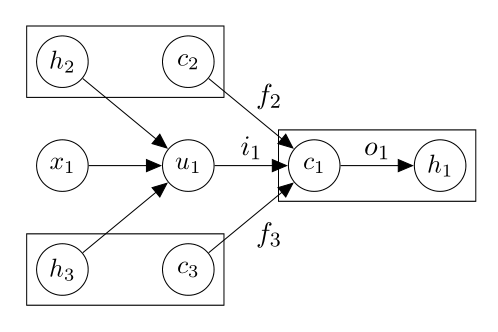
\includegraphics[height=5cm]{tree-lstm.png}
  \caption{Пример подключения узла Tree LSTM к дочерним узлам. $h_2$, $c_2$, $h_3$, $c_3$ --- состояния двух дочерних узлов, $h_1$, $c_1$ --- состояние узла родителя. $x_1$ --- входной вектор узла.}\label{fig:overview:tree_lstm}
\end{figure}

Дерево зависимостей для задачи классификации отличается тем, что каждый узел дерева содержит вектор слова. Так же дерево не является бинарным --- каждый узел может иметь произвольное количество детей. Для обработки подобных деревьев была разработана модель Tree LSTM, которая существует в двух модификациях: $N$-арная Tree LSTM, для деревьев составляющих и Child-Sum Tree LSTM, для работы с деревьями зависимостей. В данной работе была реализована модель Child-Sum Tree LSTM.\cite{tree_lstm}

Итак, ячейка Child-Sum Tree LSTM в некотором узле дерева принимает на вход состояния дочерних узлов. Пример подключения показан на рисунке~\ref{fig:overview:tree_lstm}. Состояние ячейки Tree LSTM, как и в обычной LSTM, описано двумя векторами: $h_j$ и $c_j$ --- значение скрытого слоя и внутреннего состояния соответственно. Состояние для узла $j$, имеющего множество детей $C(j)$ можно выразить следующим образом:

\begin{equation}
  \tilde{h_j} = \sum_{k\in{C(j)}}h_k,
\end{equation}
\begin{equation}
  i_j = \sigma(W^{(i)}\cdot{x_j} + U^{(i)}\cdot{\tilde{h_j}} + b^{(i)}),
\end{equation}
\begin{equation}
  \label{eq:overview:tree_lstm:forget}
  f_{jk} = \sigma(W^{(f)}\cdot{x_j} + U^{(f)}\cdot{h_k} + b^{(f)}),
\end{equation}
\begin{equation}
  o_j = \sigma(W^{(o)}\cdot{x_j} + U^{(o)}\cdot{\tilde{h_j}} + b^{(o)}),
\end{equation}
\begin{equation}
  u_j = \tan(W^{(u)}\cdot{x_j} + U^{(u)}\cdot{\tilde{h_j}} + b^{(u)}),
\end{equation}
\begin{equation}
  c_j = i_j\odot{u_j} + \sum_{k\in{C(j)}}f_{jk}\odot{c_k},
\end{equation}
\begin{equation}
  h_j = o_j\odot{\tan(c_j)},
\end{equation}
\begin{explanationx}
\item [где] $k\in{C(j)}$ для выражения~\ref{eq:overview:tree_lstm:forget}.
\end{explanationx}

В результате обработки всего дерева будет получен плотный вектор предложения.

\subsection{Классификация}
Последним этапом NLP-конвейера будет классификация плотных векторов предложений, полученных в результате сжатия. Стоит отметить, что плотные вектора предложений кодируют различные семантические свойства этих предложений, а значит с их помощью можно решать различные задачи классификации. Например сравнивать предложения по значению, похожи ли они, или противоположны, либо же нейтральны. Однако в данной работе интересная задача оценки тональности текста.\cite{Goodfellow-et-al-2016}

Для оценки тональности обычно обучают простейшую регрессионную модель

\begin{equation}
  p_{\Theta}(y|x_j) = softmax(W\cdot{h_j} + b),
\end{equation}
\begin{equation}
  y_j = \arg \max_y(p_{\Theta}(y|x_j)),
\end{equation}
\begin{explanationx}
\item[где] $h_j$ --- это плотный вектор предложения;
\item$\arg \max_y$ --- функция, которая вернет индекс максимального элемента вектора.
\end{explanationx}